\begin{frame}[plain]
\frametitle{Perspectiva general}
%------------------------------
\begin{columns}

    \pgfsetfillopacity{0.2}

    \begin{column}{0.50\textwidth}
    \vspace{-5pt}
    \begin{block}{\textcolor{cyan}{Oferta}}
        \begin{column}{0.1\textwidth}
        \vspace{-10pt} % estos espacios negativos son claves para alinear
            \tiny
            \begin{align*}
            c_{1,t}+\Phi_t \le y\\
            c_{2,t+1}\le\Phi_{t+1}^R\\
            N_{t-1}\textcolor{red}{x_t} \cdot \Phi_{t-1}^{\textbf{DLT}}=N_t(*)
            \end{align*}
        \end{column}
        \begin{column}{0.35\textwidth}  
            \begin{figure}[H]
            \begin{center}
             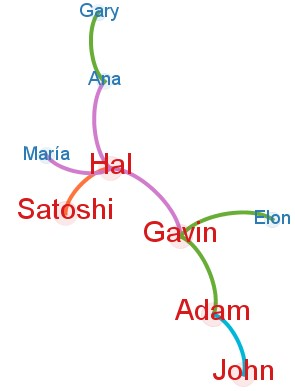
\includegraphics[width=1\textwidth]{images/C2/c2_simul_red5.jpg}
             \end{center}
            \end{figure}
            \end{column}
    \end{block}
    
    \pgfsetfillopacity{1}
    
    \begin{block}{\textcolor{dgreen}{Demanda}}
        \vspace{-10pt}
            \tiny
              \begin{align*}
              v_{t}^{\$}{M_{t}^{\$}}&={N_{t}^{\$}\left(*\right)}+(1-\lambda_t){N_{t}^{\$}\left(*\right)}\\
              v_{t}^{\bitcoinA}{M_{t}^{\bitcoinA}}&={N_{t}^{\bitcoinA}\left(*\right)+\lambda_tN_{t}^{\$}\left(*\right)}\\
              \lambda_t&=\textcolor{blue!70}{S}(\textcolor{red}{\mu_t})
            \end{align*}
    \vspace{-20pt}
            \begin{figure}[t!]
            \begin{center}
            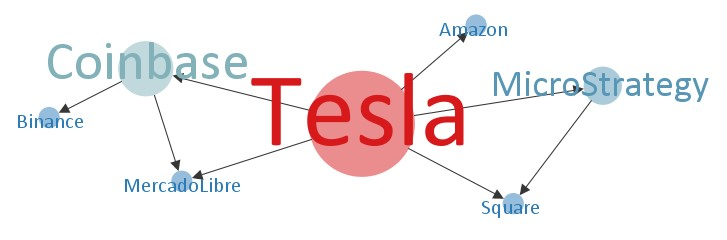
\includegraphics[width=0.6\textwidth]{images/C3/c3_simul_influ3.jpg}
             \end{center}
            \end{figure}
            
    \end{block}
    \end{column}
    
    \begin{column}{0.55\textwidth}
    
    \pgfsetfillopacity{0.2}
    
    \begin{block}{Implicancias}
    \tiny

    \begin{align*}
    v^{\$a}_1 M^{\$a}_1&=P_1^{{\$a}} + \lambda_1 (1-\alpha_1) R_1^{{\$a}} + (1-\lambda_1) \textcolor{blue!60}{\rho_1}  R_1^{{\$a}}\\
    v_1^{\$} M_1^{\$}&=(1-\lambda_1) \textcolor{green!70}{\delta_1} R_1^{\$a}\\
    v_1^{\bitcoinA} M_1^{\bitcoinA}&=\textcolor{orange}{\lambda_1}  \alpha_1 R_1^{\$a} + (1-\lambda_1) \textcolor{red}{\beta_1} R_1^{\$a}\\
    e_t^{{\$a};{\$}}&=\frac{v_1^{\$a}}{v_1^{\$}}
    \end{align*}
    
    \vspace{-5pt}
    
    \begin{figure}[H]
    \begin{center}
     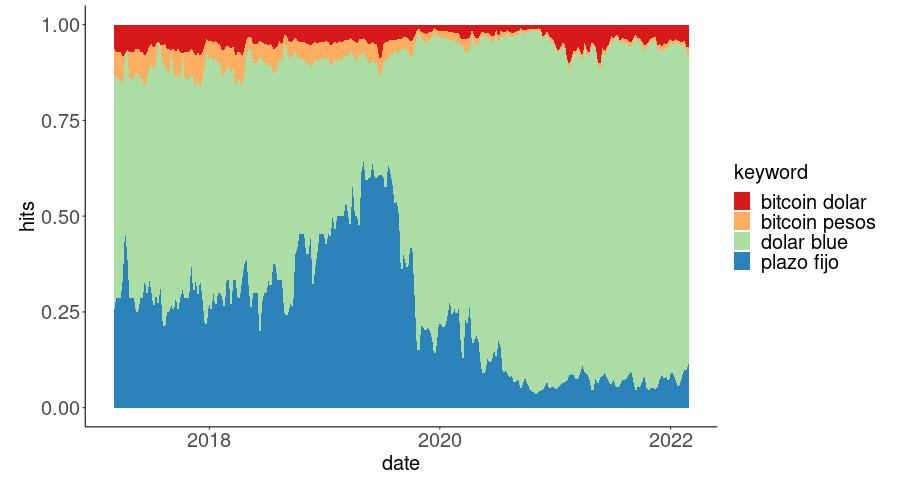
\includegraphics[width=1\textwidth]{images/C4/Rplot001.png}
     \end{center}
    \end{figure}
    
    \pgfsetfillopacity{1}
    
    \end{block}

    \end{column}
\end{columns}

\note{
\begin{itemize}
    \item Finalizada la primera parte de la investigación, volvemos a la filmina que presenta el panorama general. 
    \item Comenzamos con el análisis de la segunda parte de la investigación asociado a los motivos de demanda de bitcoin. 
\end{itemize}
}

\end{frame}
%----------

\subsection{Objetivos}
%---------------------
\begin{frame}{}

    \textcolor{blue}{\textbf{Objetivo}}.\\
    \vspace{5mm}
    \begin{itemize}
        \setlength\itemsep{1em}
        \item[] Analizar los \textcolor{blue}{motivos de demanda} de bitcoin. 
        \item[] Construir un \textcolor{blue}{modelo} que explique la demanda de bitcoin a partir del comportamiento de un grupo de \textcolor{blue}{influenciadores} y de un grupo de \textcolor{blue}{seguidores}. 
        \item[] Evaluar empíricamente el modelo propuesto a partir de \textcolor{blue}{datos estimados de las redes sociales}. 
    \end{itemize}
 
    \vspace{5mm}
    \textcolor{dgreen}{\textbf{Conjetura}}. 
    \vspace{5mm}
    \begin{itemize}
    \item[] La \textcolor{dgreen}{demanda de bitcoin} \textcolor{dgreen}{se encuentra asociada} de las opiniones de un grupo de \textcolor{dgreen}{actores influyentes} del mercado, de la opinión de los reguladores y del comportamiento de un grupo de seguidores. 
    \end{itemize}


\note{
\begin{itemize}
    \item Para esta segunda parte de la investigación, se plantean tres objetivos específicos
    \item (Leer cada objetivo)
    \item A su vez, se plantea la siguiente conjetura:
    \item (Leer la conjetura)
\end{itemize}
}
    
\end{frame}
%----------

\subsection{Definiciones}
%------------------------
\begin{frame}

\begin{displayquote}
\small
Las \textcolor{blue}{creencias} son importantes; si los jóvenes de un determinado período renuncian a algo de sus bienes por dinero, es porque piensan que la siguiente generación también lo hará.
\end{displayquote}
\raggedleft {\cite{Garratt2018},\\ \citetitle{Garratt2018}}

\vspace{5mm}
\begin{block}<2>{Creencias}
La demanda de un activo como activo monetario depende de las \textcolor{blue}{expectativas} en torno a que dicho activo pueda cumplir en el futuro con las \textcolor{blue}{funciones de medio de pago, reserva de valor y unidad de cuenta}. 
\end{block}

\note{
\begin{itemize}
    \item Para esta segunda parte de la investigación se propone retomar algunos conceptos asociados al valor del dinero fiduciario.
    \item En este sentido, \textbf{Garrat y Wallace} indican que (leer cita)
    \item A partir de esa definición, se propone el siguiente concepto de creencias (leer el recurado sobre DLT)
    \item En este sentido, por un lado, bitcoin se asemeja a las formas de dinero fiduciario actuales (como se indicó en la primera parte de la investigación). 
    \item Y, por otro, bitcoin se diferencia de los activos monetarios con valor intrínseco, como el oro, cuya demanda se encuentra vinculada, además, a su utilidad como bien de uso. 
\end{itemize}
}
    
\end{frame}
%----------

\begin{frame}

\begin{displayquote}
\small
Nada puede haber sido tan favorable a la génesis de un medio de cambio como la aceptación, por parte de \textcolor{blue}{los sujetos económicos más perspicaces y capaces}, para su propio beneficio económico, y durante un período de tiempo considerable, de bienes eminentemente vendibles con preferencia a todos los demás. 
\end{displayquote}
\raggedleft \href{https://www.jstor.org/stable/2956146}{\cite{Menger1892},\\ \citetitle{Menger1892},\\Sección VI}

\vspace{5mm}
\begin{block}<2>{Infuenciadores}
Los \textcolor{dgreen}{influenciadores} son \textcolor{blue}{actores} que \textcolor{blue}{generan información} nueva. Son actores que cuentan con \textcolor{blue}{más información} y \textcolor{blue}{mejor capacidad de análisis} que el resto de los demandantes del mercado. Son quienes determinan la tendencia de precios en el largo plazo. 
\end{block}

\note{
\begin{itemize}
    \item Una segunda idea relevante para esta segunda parte de la investigación es la que distingue a ciertos grupos por sobre el resto al momento de determinar que activos funcionarán como medios de intercambio. 
    \item En este sentido, por ejemplo, Menger, en una publicación muy influyente sobre el origen del dinero indica que (leer cita).
    \item A partir de estas ideas de Menger, se propone definir a los actores influyentes como (leer recuadro)
\end{itemize}
}
    
\end{frame}
%----------

\begin{frame}

\begin{displayquote}
La sabiduría mundana enseña que es mejor para la \textcolor{blue}{reputación} \textcolor{blue}{fracasar convencionalmente} que tener éxito de forma no convencional.
\end{displayquote}
\raggedleft \cite{Keynes1936TheExpectation} \\ \citetitle{Keynes1936TheExpectation}\\ Sección V

\vspace{5mm}
\begin{block}<2>{Seguidores}
Los \textcolor{dgreen}{seguidores} son los agentes que \textcolor{blue}{imitan} el comportamiento de los actores influyentes. El comportamiento de los seguidores se encuentra asociado al comportamiento en el precio de corto plazo. 
\end{block}

\note{
\begin{itemize}
    \item Finalmente, otra idea relevante para esta segunda parte de la investigación se asocia al comportamiento de actores imitadores.  
    \item En este sentido, por ejemplo, Keynes, en la última parte de la sección 5 del capítulo 12 de Teoría General (sección donde se desarrollan las ideas del concurso de belleza) indica que (leer cita).
    \item A partir de estas ideas de Keynes, se propone definir a los seguidores como (leer recuadro)
\end{itemize}
}
    
\end{frame}
%----------

\subsection{Evaluación conceptual y empírica}
%-----------------------------------------------

% overview
\begin{frame}{Evaluación conceptual y empírica}
    
    \begin{block}{Modelo}
    
    \begin{minipage}[t][.20\textheight][t]{\textwidth}

        \begin{column}{0.30\textwidth}
            \tiny
            \begin{align*}
            v_{t}^{\$}{M_{t}^{\$}}&=     N_{t}^{\$}(y_{t}^{\$}-c_{t}^{\$})
            (1-\lambda_t)\\
            v_{t}^{\bitcoinA}{M_{t}^{\bitcoinA}}&=N_{t}^{\bitcoinA}(y_{t}^{\bitcoinA}-c_{t}^{\bitcoinA})+{N_{t}^{\$}(y_{t}^{\$}-c_{t}^{\$})}\lambda_t\\
            {\lambda_t}&={S}({\mu_t})
            \end{align*}
        \end{column}
        \begin{column}{0.45\textwidth}
        
        \end{column}
        
    \end{minipage}
    \end{block}

\begin{block}{Evaluación empírica}
    
    \begin{minipage}[t][.40\textheight][t]{\textwidth}

\begin{column}{0.3\textwidth}
    \tiny
    \begin{figure}[H]
        \begin{center}
             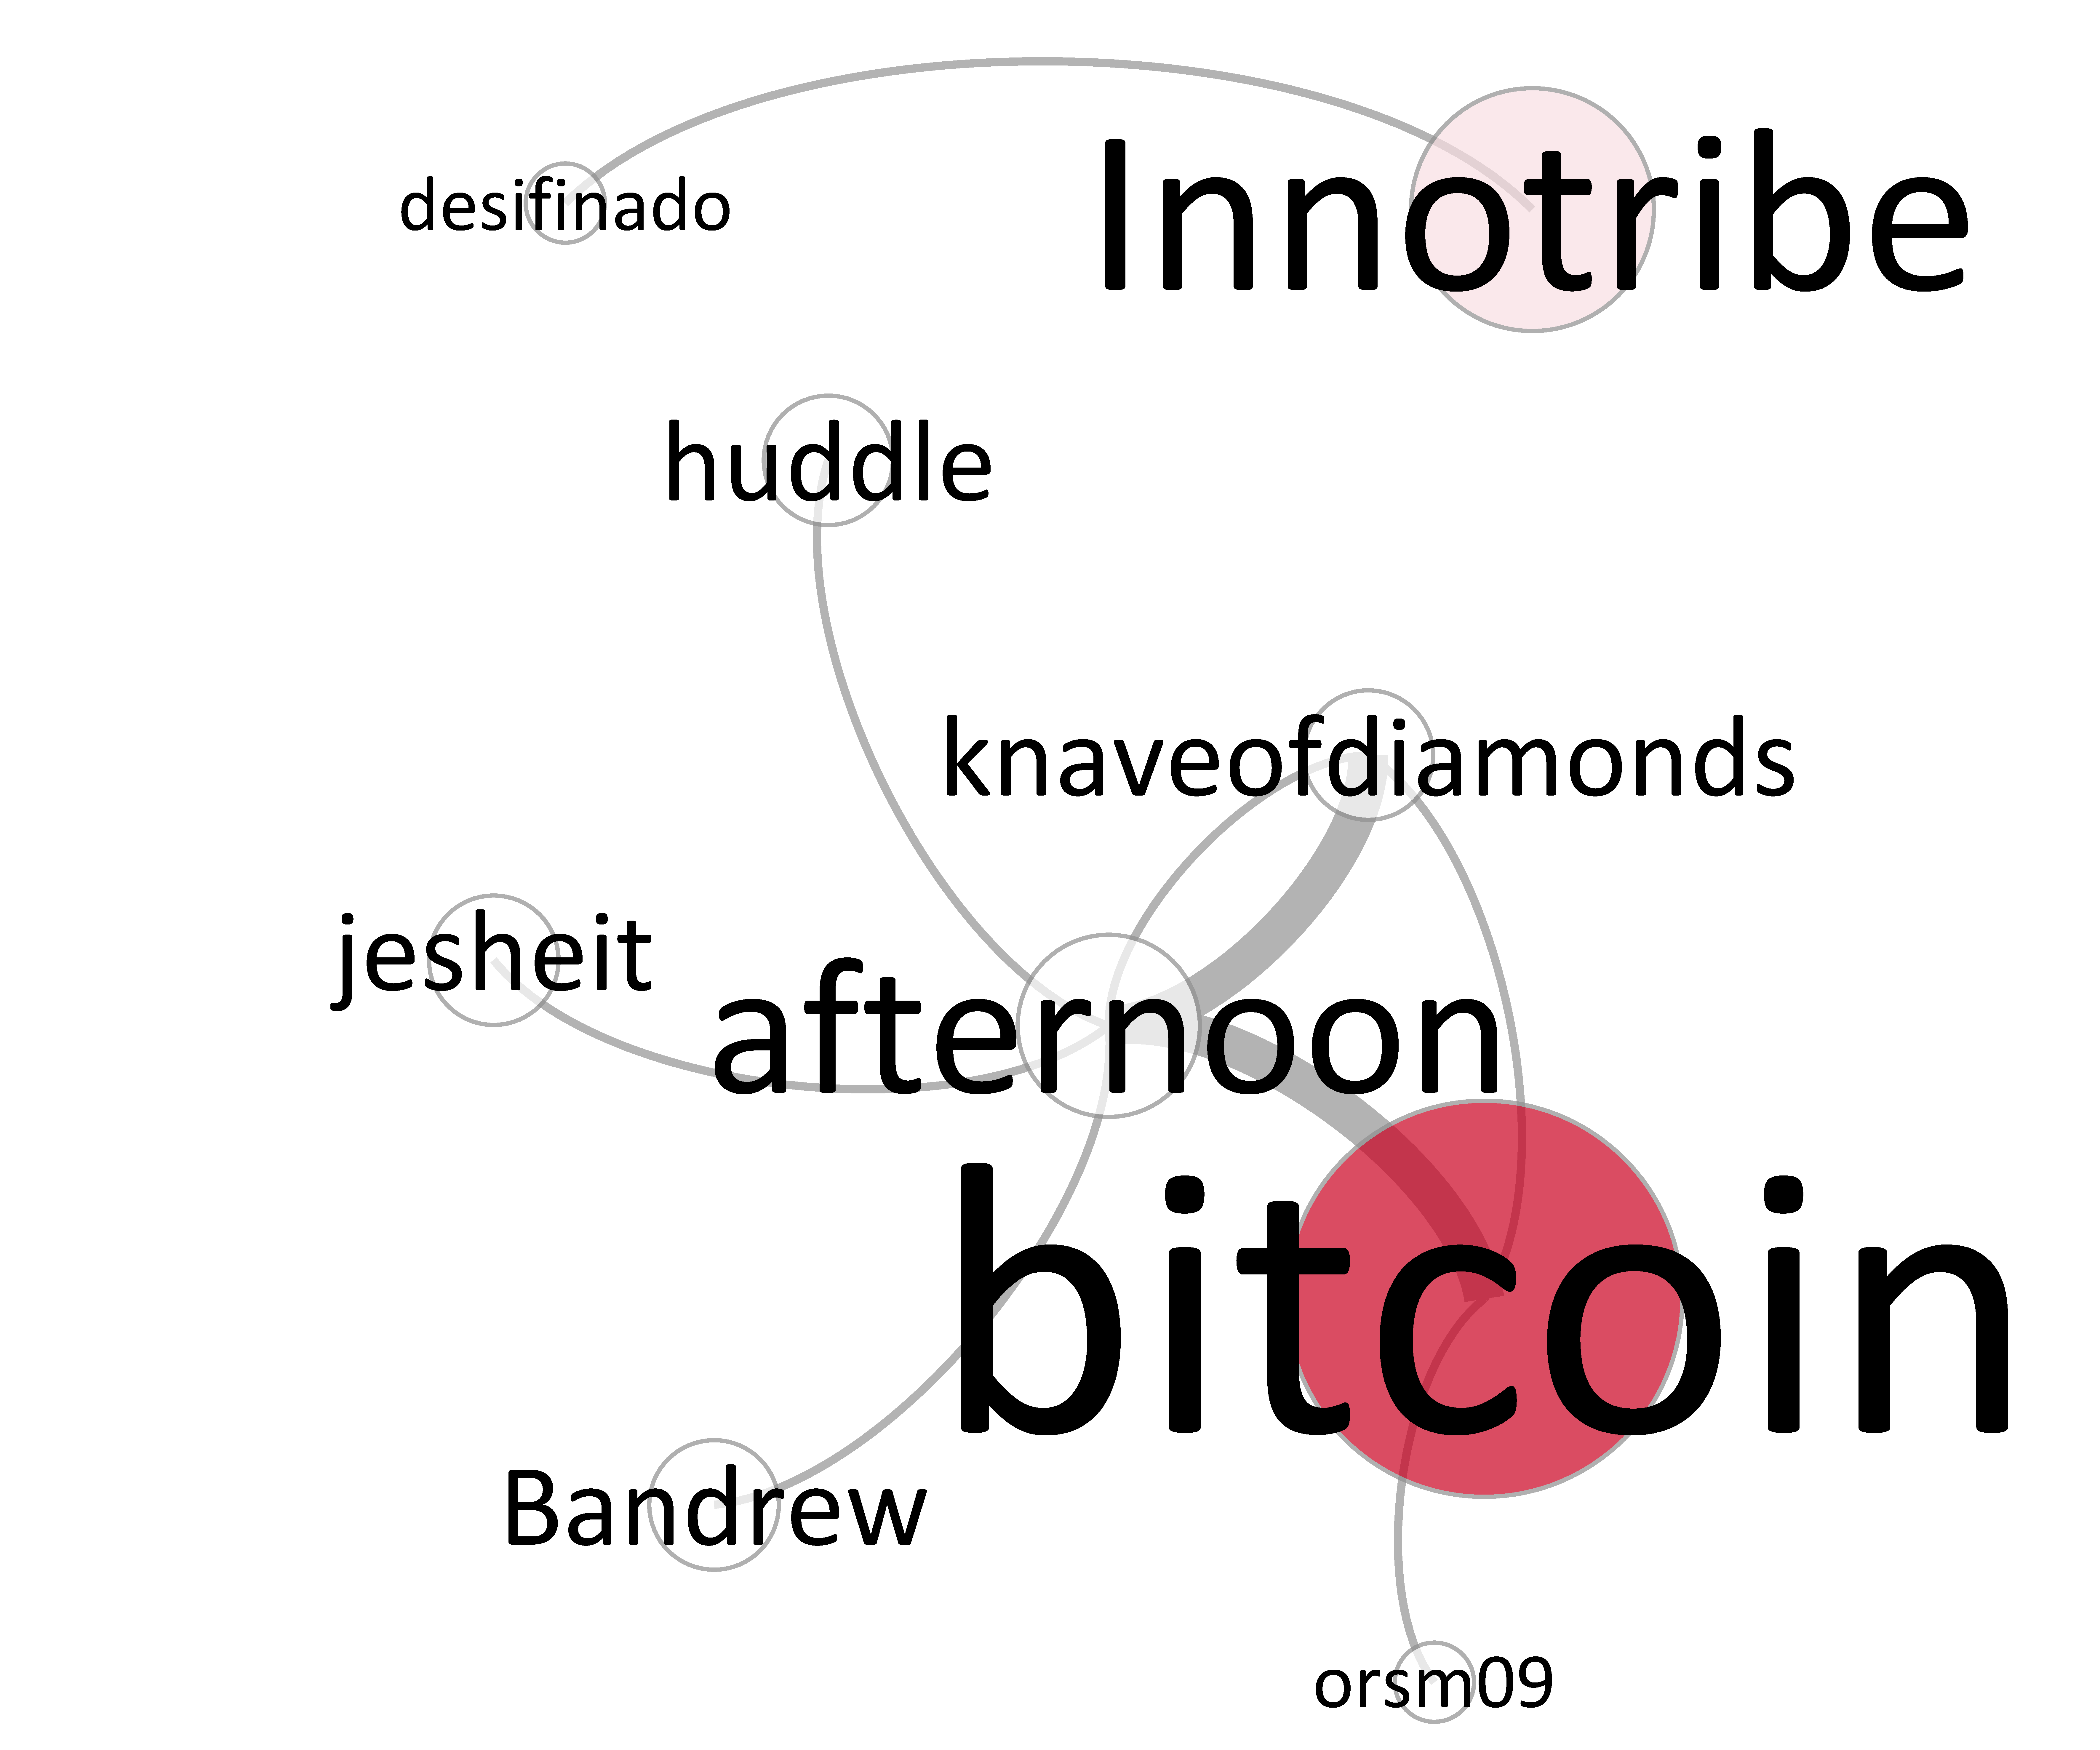
\includegraphics[width=1\textwidth]{images/C3/c3_red_influ_real.pdf}
         \end{center}
    \end{figure}
\end{column}
\begin{column}{0.3\textwidth}  
    \tiny
    \begin{figure}[H]
        \begin{center}
         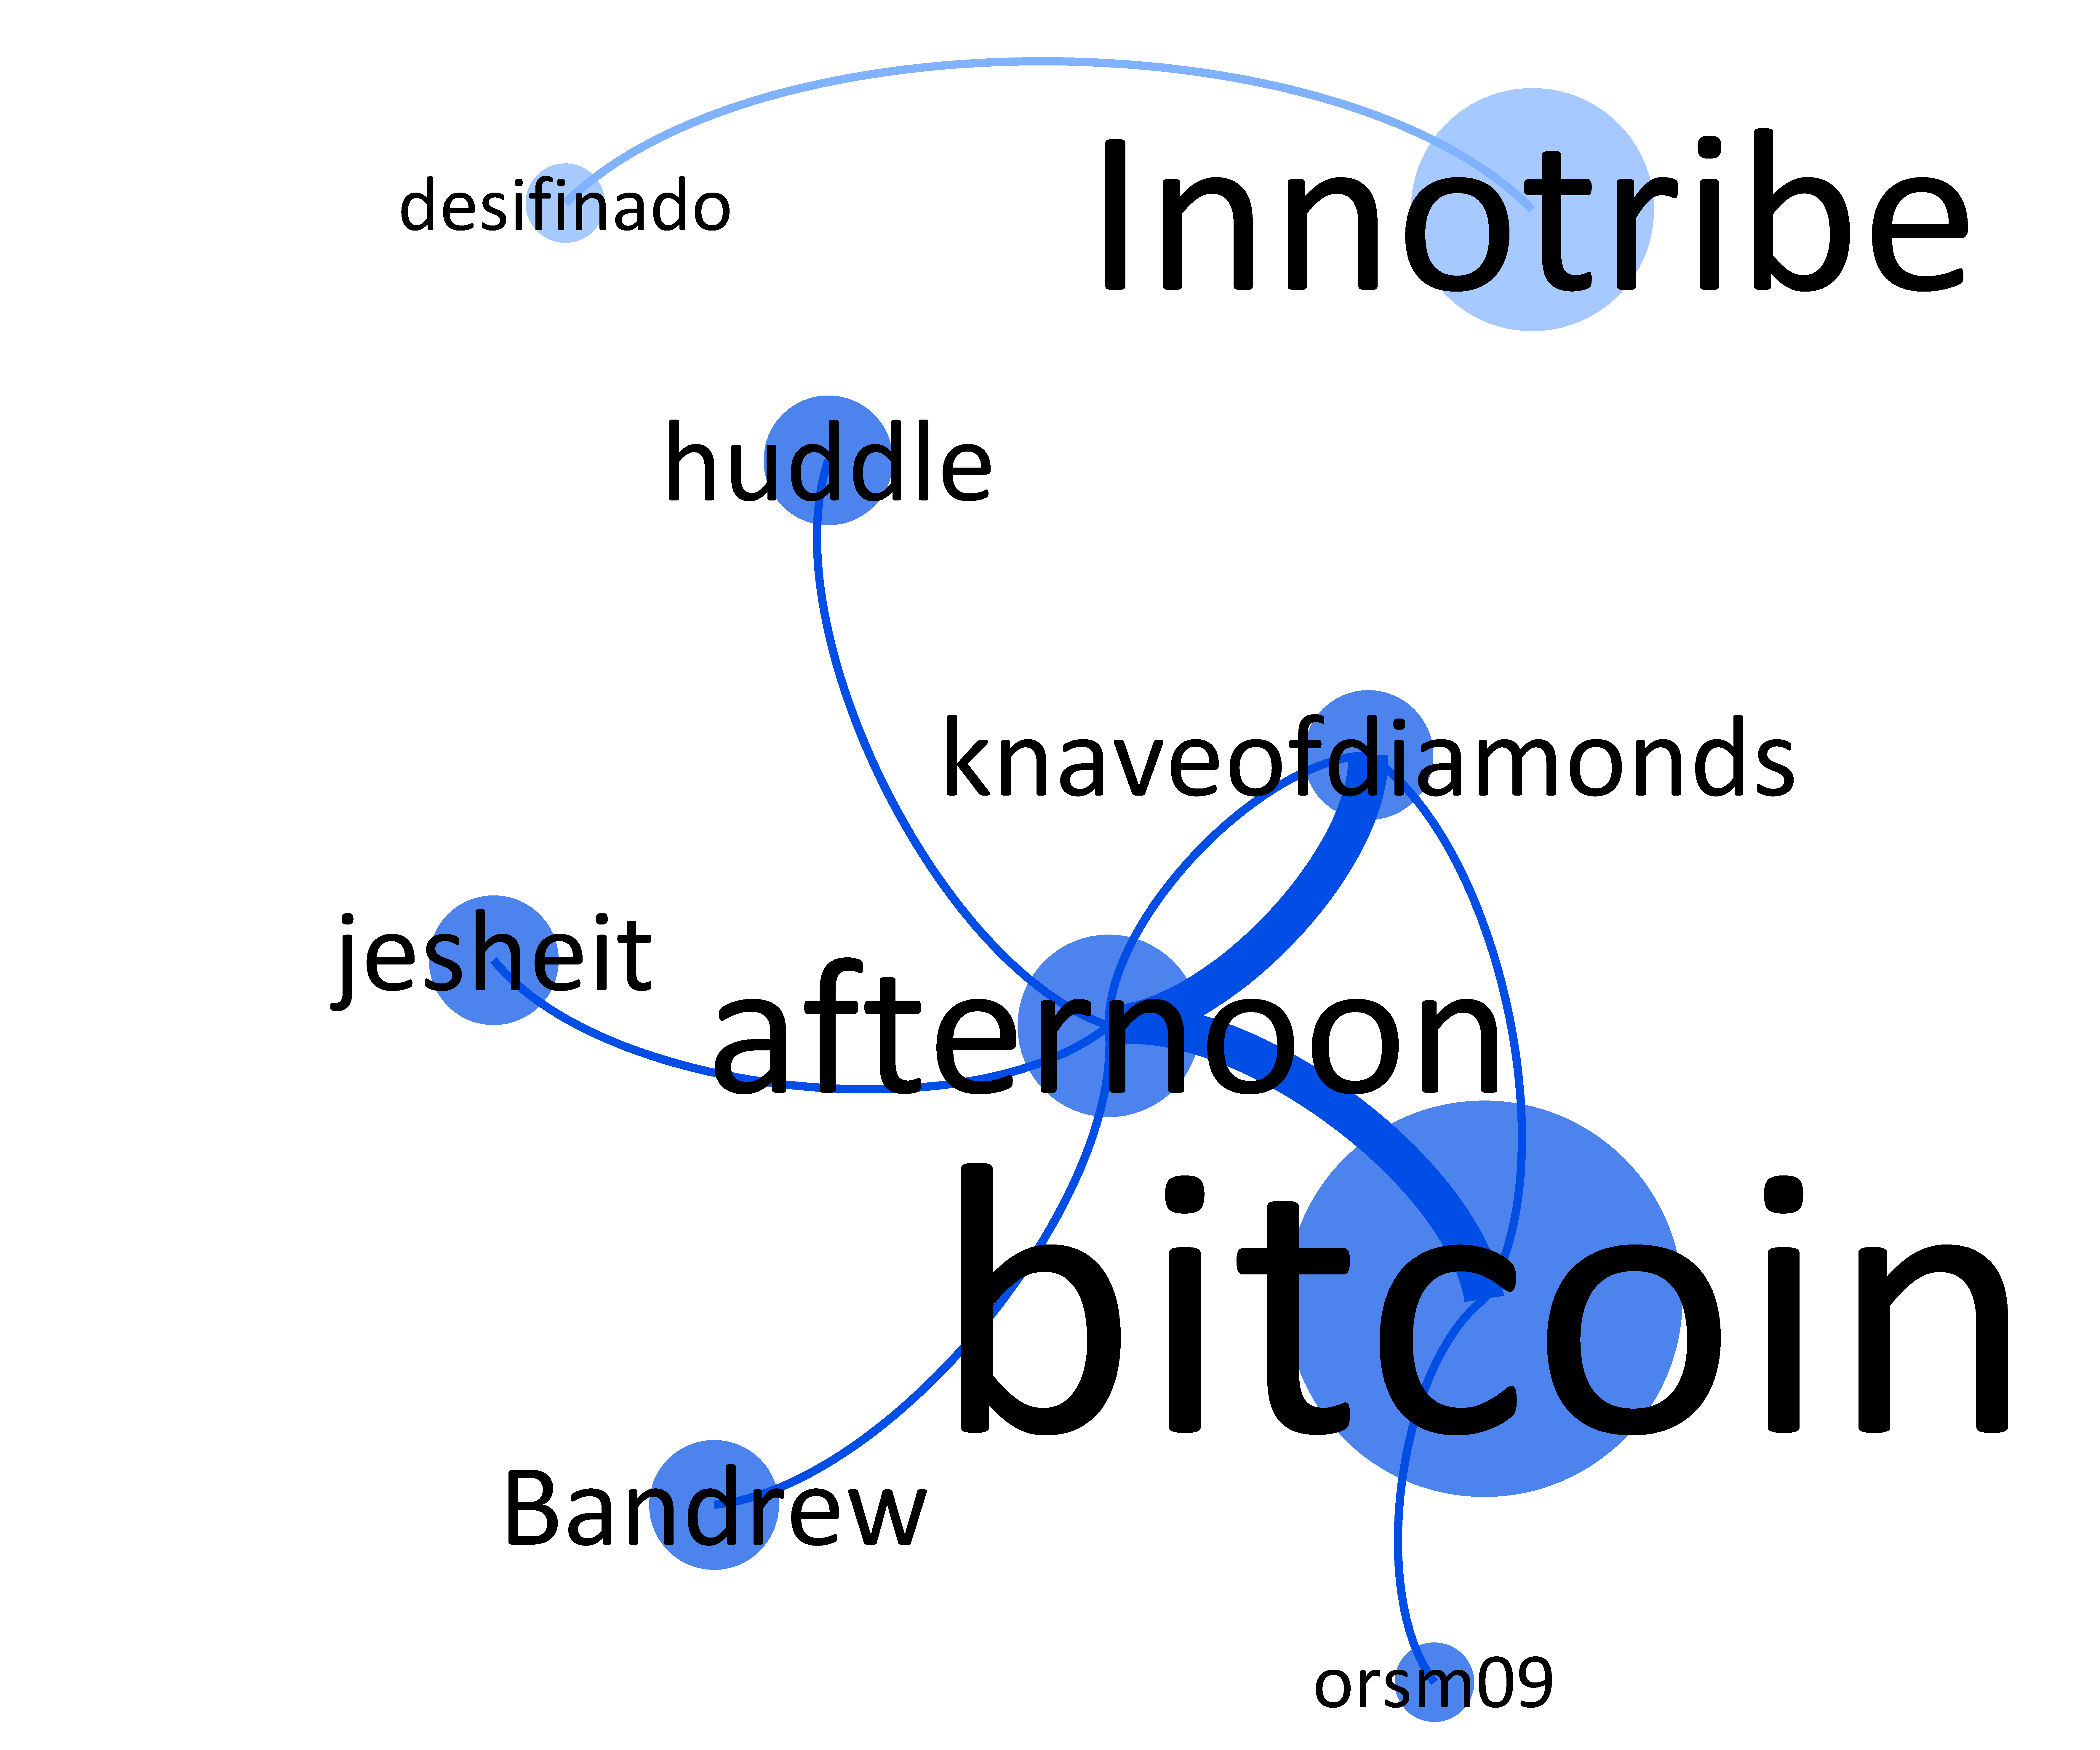
\includegraphics[width=1\textwidth]{images/C3/c3_red_comunidades_real.pdf}
         \end{center}
    \end{figure}
\end{column}
\begin{column}{0.3\textwidth}  
    \tiny
    \begin{figure}[H]
        \begin{center}
         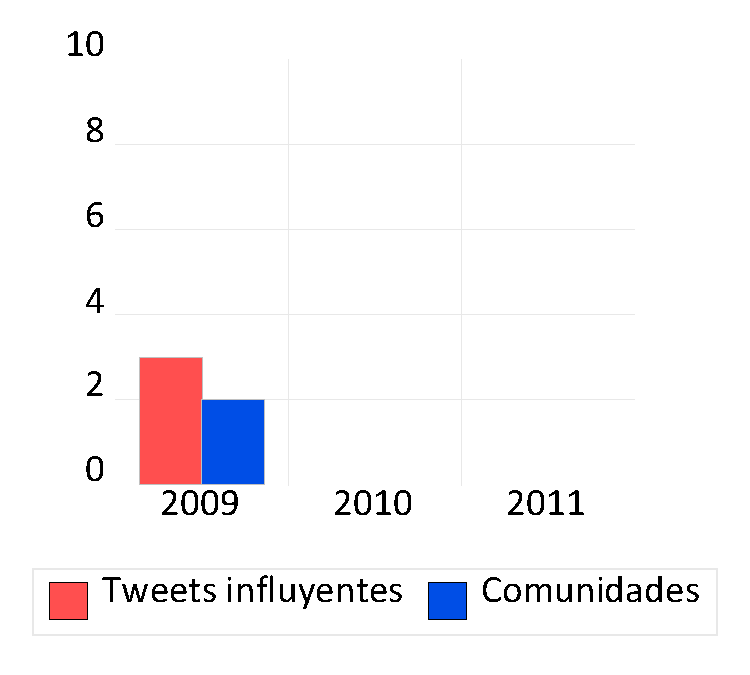
\includegraphics[width=1\textwidth]{images/C3/c3_timesseries_2009_real.pdf}
         \end{center}
    \end{figure}
\end{column}

    \end{minipage}

\end{block}

\note{
\begin{itemize}
    \item Para esta segunda parte de la investigación se propone: 
    \item Evaluación conceptual: modelo generaciones superpuestas con dos activos monetarios (dinero fiduciario y bitcoin) y dos actores (influyentes y seguidores). 
    \item De manera alternativa, se propone una explicación desde la teoría de juegos con un juego simultáneo con información perfecta. En este juego existe la posibilidad de equilibrios múltiples bajo problemas de coordinación. El análisis desde la teoría de juegos se encuentra en el anexo GameTheory.
    \item Evaluación empírica: análisis con técnicas de red a partir de mensajes de la red social twitter
    \end{itemize}
}

\end{frame}
% slides del modelo con overlay

\begin{frame}[t]
\frametitle{Evaluación conceptual y empírica}
    
    \begin{block}{Modelo}
    
    \begin{minipage}[t][.20\textheight][t]{\textwidth}

        \begin{column}{0.30\textwidth}
            \tiny
            \begin{align*}
            \onslide<2,4>{v_{t}^{\$}{M_{t}^{\$}}}&=      \onslide<3,4,6>{N_{t}^{\$}(y_{t}^{\$}-c_{t}^{\$})}\onslide<6>{(1-\lambda_t)}\\
            \onslide<5>{v_{t}^{\bitcoinA}{M_{t}^{\bitcoinA}}}&=
            \onslide<5>{N_{t}^{\bitcoinA}(y_{t}^{\bitcoinA}-c_{t}^{\bitcoinA})}+
            \onslide<6>{{N_{t}^{\$}(y_{t}^{\$}-c_{t}^{\$})}\onslide<6>{\lambda_t}}\\
            \only<7|handout:0>{{\lambda_t}&={S}({\mu_t})}
            \only<8>{{\lambda_t}&={S}(\textcolor{red}{\mu_t})}
            \only<9|handout:0>{{\lambda_t}&=\textcolor{blue!70}{S}({\mu_t})}
            \end{align*}
        \end{column}
        \begin{column}{0.45\textwidth}
        \only<2|handout:0>{
                    \tiny
                    \justify
                    Oferta de dinero fiduciario
                    \begin{itemize}
                        \item $v_t^{\$}$: valor de una unidad del act
                        ivo fiduciario en término de bienes;
                        \item $M_t^{\$}$: oferta de activo fiduciario.
                    \end{itemize}
                    }
        
        \only<3|handout:0>{
                    \tiny
                    \justify
                    Demanda de dinero fiduciario
                    \begin{itemize}
                        \item $y_t^{\$}$: asignación de bienes
                        \item $c_t^{\$}$: consumo
                        \item $N_t^{\$}$: cantidad de personas
                    \end{itemize}
                    }
                    
        \only<4|handout:0>{
                    \tiny
                    \justify
                    Mercado de dinero fiduciario
                    }

        \only<5|handout:0>{
                    \tiny
                    \justify
                    Mercado de dinero criptográfico
                    }
        
        \only<6|handout:0>{
                    \tiny
                    \justify
                    Sustititución monetaria
                    }
        
        \only<7|handout:0>{
                    \tiny
                    \justify
                    Parámetro de grado de influencia
                    \begin{itemize}
                        \item $\mu_t$ influenciadores
                        \item $S$ seguidores
                    \end{itemize}
                    }
        
        \only<8>{
                    \tiny
                    \justify
                    Parámetro de grado de influencia
                    \begin{itemize}
                        \item $\mu_t$ \textcolor{red}{influenciadores}
                        \item $S$ seguidores
                    \end{itemize}
                    }
                    
        
        \only<9|handout:0>{
                    \tiny
                    \justify
                    Parámetro de grado de influencia
                    \begin{itemize}
                        \item $\mu_t$ influenciadores
                        \item $S$ \textcolor{blue!70}{seguidores}
                    \end{itemize}
                    }
        
        \end{column}
        
    \end{minipage}
    \end{block}

\begin{block}{Evaluación empírica}

\begin{minipage}[t][.40\textheight][t]{\textwidth}
    
\begin{column}{0.3\textwidth}
    \tiny
    \begin{figure}[H]
        \begin{center}
             \includegraphics<8,9>[width=1\textwidth]{images/C3/c3_red_influ_real.pdf}
         \end{center}
    \end{figure}
\end{column}
\begin{column}{0.3\textwidth}  
    \tiny
    \begin{figure}[H]
        \begin{center}
         \includegraphics<9>[width=1\textwidth]{images/C3/c3_red_comunidades_real.pdf}
         \end{center}
    \end{figure}
\end{column}
\begin{column}{0.3\textwidth}  
    \tiny
    \begin{figure}[H]
        \begin{center}
         \includegraphics<8|handout:0>[width=1\textwidth]{images/C3/c3_timesseries_2009_real_v02.pdf}
        \includegraphics<9>[width=1\textwidth]{images/C3/c3_timesseries_2009_real.pdf}
         \end{center}
    \end{figure}
\end{column}

\end{minipage}
\end{block}

\note{
\small
\begin{itemize}
    \item 1° Economía con un activo monetario fiduciario.
    \item 2° Creación de una nueva moneda digital. Uso limitado
    \item 3° Sustitución 
    \item De la fracción de ciudadanos que elija el activo digital y, por lo tanto, el activo fiduciario, estará asociada al comportamiento de un grupo de actores influyentes y de un grupo de seguidores
    \item Se define, por lo tanto, el parámetro de grado de influencia como: $\lambda_t=S(\mu_t)$; $\mu_t$: parámetro interés del grupo de actores influyentes; $S$ función indica comportamiento de imitación de seguidores. El parámetro $\mu_t$ depende, a su vez, del interés de actores influyentes de mercado y del regulador. La función $S$ amplifica el interés reflejado por parte de los influenciadores. 
\end{itemize}
}

\end{frame}

% slides de evaluación empírica 2010 2 de 2

\begin{frame}[t]
\frametitle{Evaluación conceptual y empírica}
    
    \begin{block}{Modelo}
    
    \begin{minipage}[t][.20\textheight][t]{\textwidth}

        \begin{column}{0.30\textwidth}
            \tiny
            \begin{align*}
            v_{t}^{\$}{M_{t}^{\$}}&=     N_{t}^{\$}(y_{t}^{\$}-c_{t}^{\$})
            (1-\lambda_t)\\
            v_{t}^{\bitcoinA}{M_{t}^{\bitcoinA}}&=N_{t}^{\bitcoinA}(y_{t}^{\bitcoinA}-c_{t}^{\bitcoinA})+{N_{t}^{\$}(y_{t}^{\$}-c_{t}^{\$})}\lambda_t\\
            {\lambda_t}&={S}({\mu_t})
            \end{align*}
        \end{column}
        \begin{column}{0.45\textwidth}
        
        \end{column}
        
    \end{minipage}
    \end{block}

\begin{block}{Evaluación empírica}

\begin{minipage}[t][.40\textheight][t]{\textwidth}
    
\begin{column}{0.3\textwidth}
    \tiny
    \begin{figure}[H]
        \begin{center}
             \includegraphics[width=1\textwidth]{images/C3/c3_red_influ_real_2010.pdf}
         \end{center}
    \end{figure}
\end{column}
\begin{column}{0.3\textwidth}  
    \tiny
    \begin{figure}[H]
        \begin{center}
         \includegraphics[width=1\textwidth]{images/C3/c3_red_com_real_2010.pdf}
         \end{center}
    \end{figure}
\end{column}
\begin{column}{0.3\textwidth}  
    \tiny
    \begin{figure}[H]
        \begin{center}
         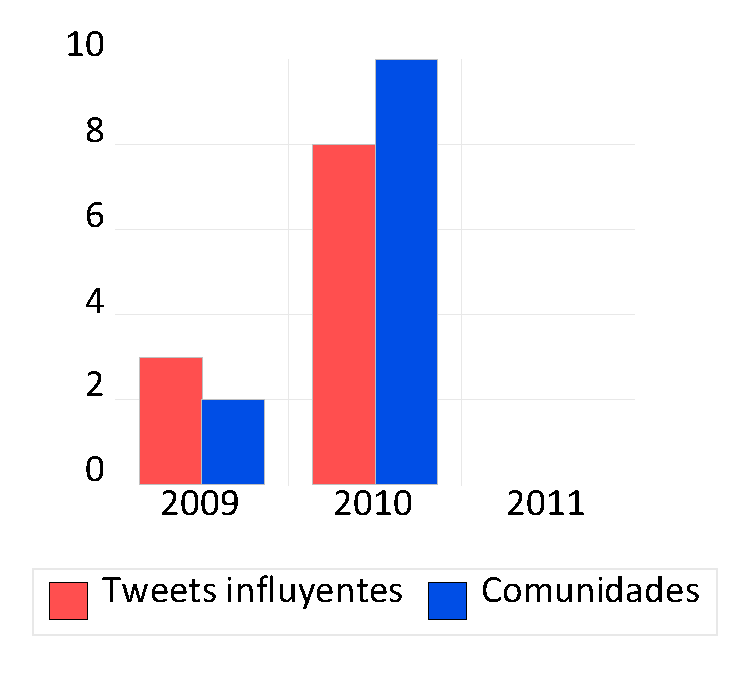
\includegraphics[width=1\textwidth]{images/C3/c3_times_series_2010.pdf}
         \end{center}
    \end{figure}
\end{column}

\end{minipage}
\end{block}

\note{
\footnotesize
\begin{itemize}
    \item La conjetura empírica indica que existe una asociación entre el valor de $\lambda$ y el valor del activo digital. 
    \item Se espera que niveles elevados de $\lambda$ estén asociados a incrementos en el valor del activo digital. 
    \item Fuente: la recopilación de datos de tweets se efectúa mediante Python
    \item Para generar la lista de \textbf{actores influyentes} (gráfico de la izq) se utiliza la métrica de pagerank que mide la importancia de cada nodo dentro del gráfico basándose en el número de relaciones entrantes y la importancia de los nodos fuente correspondientes. El supuesto subyacente es que un actor es tan importante como los actores con los que se conecta. 
    \item Para estimar el comportamiento de los \textbf{seguidores}, se estudian los mismos datos, la misma red, pero desde una dimensión diferente. Ahora se quiere evaluar la estructura de la red, su topología. Se considera que una red más densa debería propagar los mensajes de los influyentes con mayor velocidad y, por lo tanto, debería amplificar su sentido. 
\end{itemize}
}

\end{frame}
%----------

\subsection{Resultados}
%---------------------


\begin{frame}
\frametitle{Se compara la variación de \textcolor{red}{tweets influentes}...}

\begin{figure}[H]
    \begin{center}
         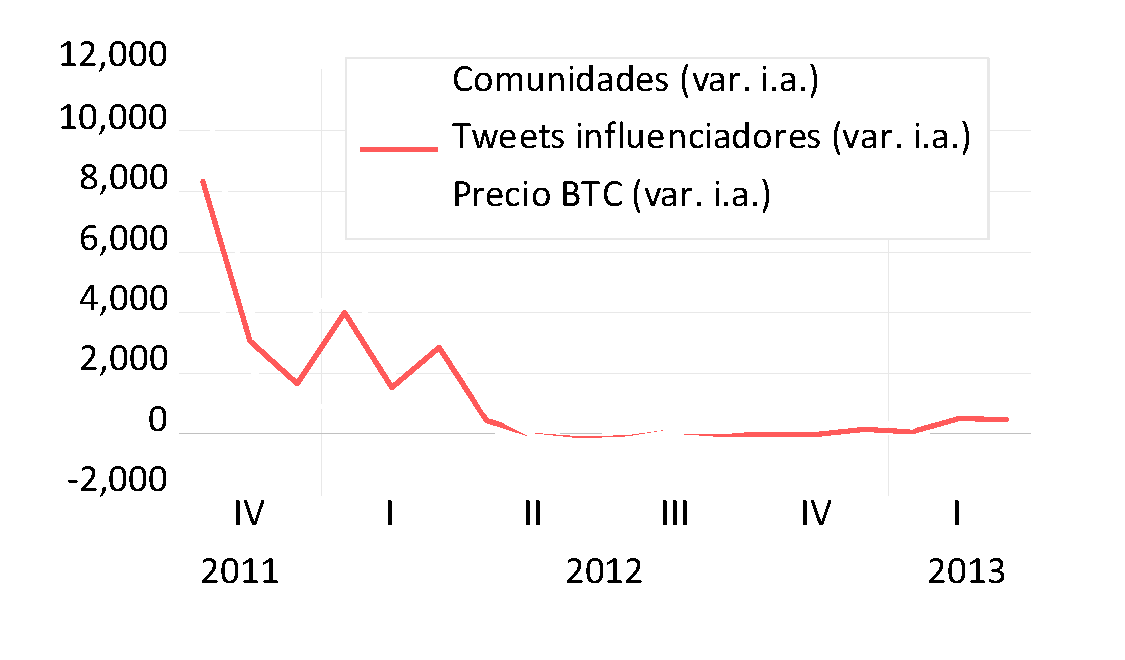
\includegraphics[width=1\textwidth]{images/C3/results/times_series_result_01.pdf}
     \end{center}
\end{figure}

\note{
\begin{itemize}
    \item Luego de estimar las variaciones asociadas a las opiniones de los actores influyentes a través del uso del algoritmo PageRank y estimar el comportamiento del grupo de seguidores a través de las métricas de red, se propone evaluar la asociación entre dichas estimaciones y el precio de bitcoin. Para estimar las relaciones entre variables se transforman las variables para obtener las variaciones interanuales. 
    \item (leer encabezado)
\end{itemize}
}

\end{frame}
%----------

\begin{frame}
\frametitle{...y la variación de \textcolor{blue}{comunidades}...}

\begin{figure}[H]
    \begin{center}
         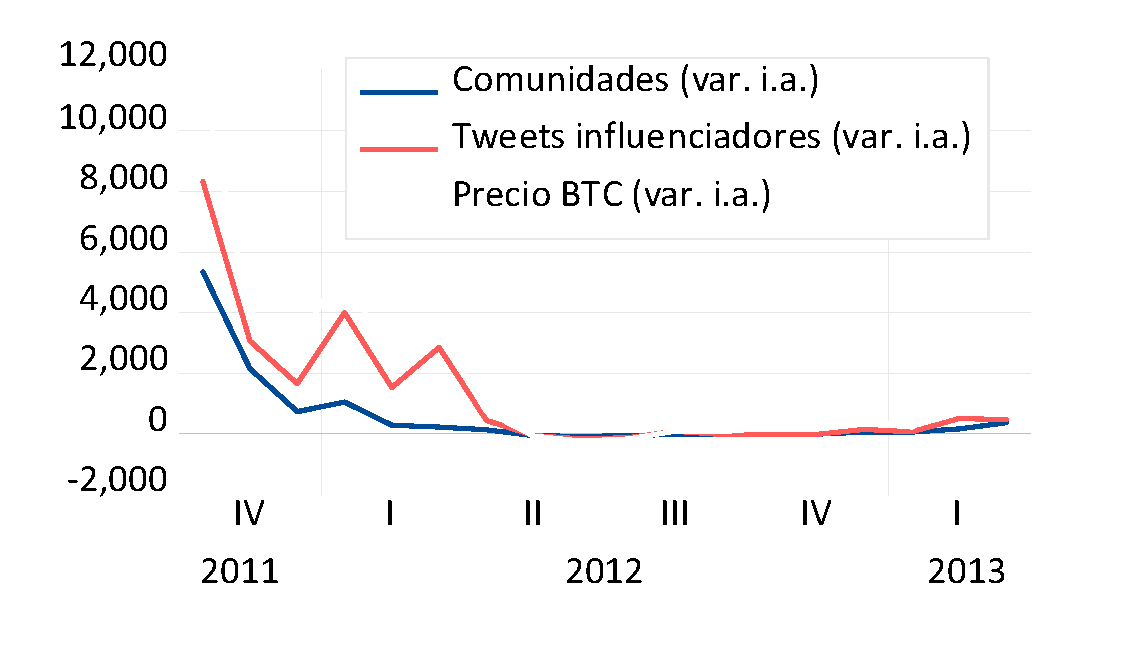
\includegraphics[width=1\textwidth]{images/C3/results/times_series_result_02.pdf}
     \end{center}
\end{figure}

\note{
\begin{itemize}
    \item (leer encabezado)
\end{itemize}
}

\end{frame}
%----------


\begin{frame}
\frametitle{con la variación en el \textcolor{dgreen}{precio}.}

\begin{figure}[H]
    \begin{center}
         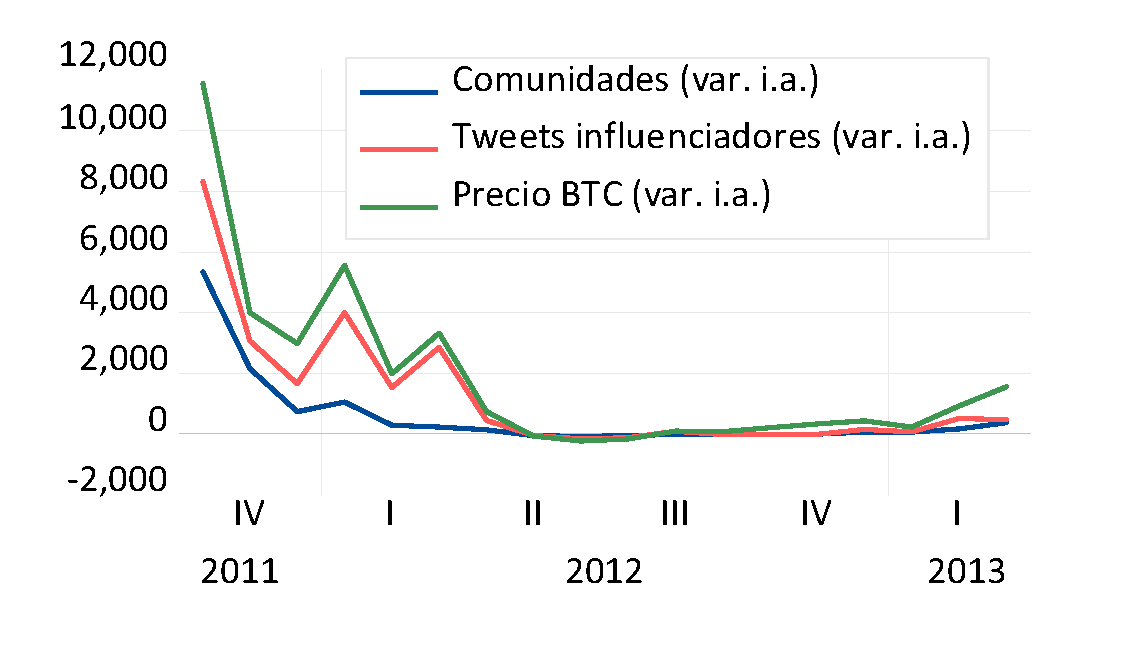
\includegraphics[width=1\textwidth]{images/C3/results/times_series_result_03.pdf}
     \end{center}
\end{figure}

\note{
\begin{itemize}
    \item (leer encabezado)
    \item La correlación entre la variación i.a. del precio de bitcoin y la variación i.a. de los tweets de los influyentes es de 0.82 y la correlación entre la variación del precio de bitcoin y la variación i.a. de los nodos es 0.94.
\end{itemize}
}

\end{frame}
%----------

% comparación con referencias actuales

\begin{frame}
\frametitle{Estos resultados se encuentran asociados a nuevas métricas de mercado}

\begin{figure}[H]
    \begin{center}
         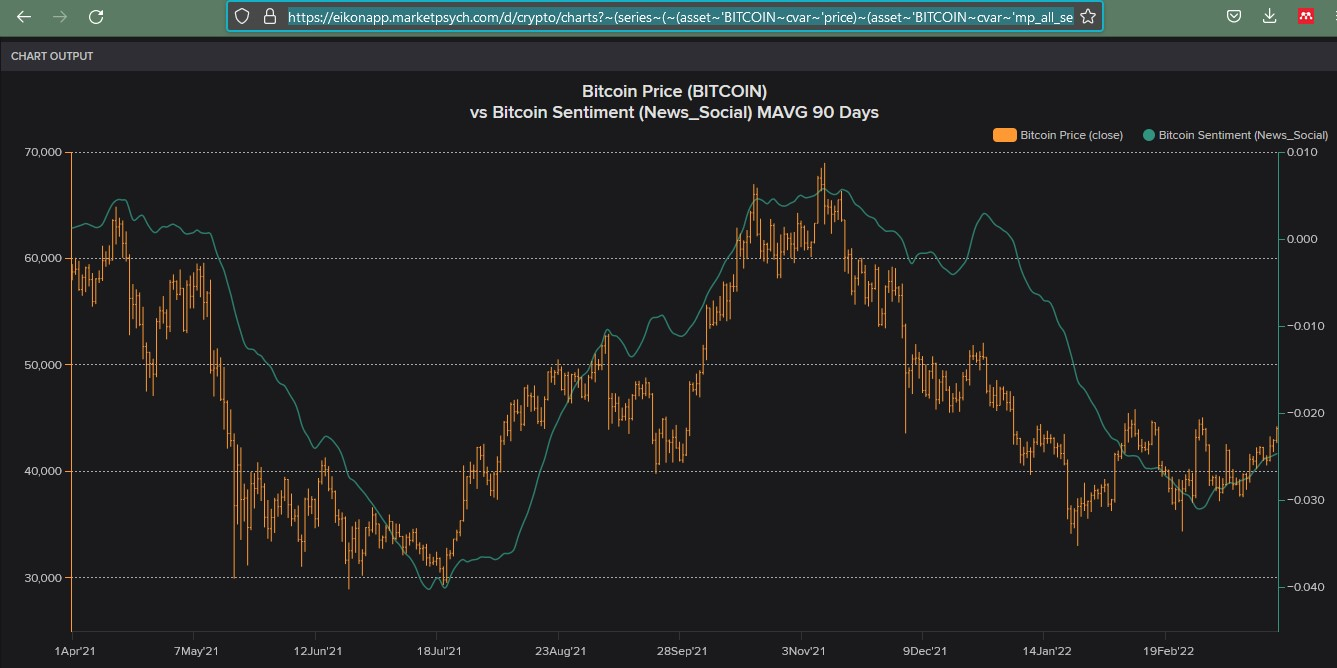
\includegraphics[width=1\textwidth]{images/C3/ref/reuters2.jpg}
     \end{center}
    \source{Fuente: \href{https://www.thomsonreuters.com/en/press-releases/2018/march/thomson-reuters-launches-bitcoin-sentiment-data-feed-for-trading-and-risk-management.html}{Thomson Reuters}}
\end{figure}

\note{
\begin{itemize}
    \item Este tipo de análisis a partir de datos de redes sociales están comenzando a ser utilizados por consultoras de mercado para evaluar la evolución del precio de bitcoin y otros activos digitales. 
    \item Este es un indicador de la empresa Thomson Reuters.
\end{itemize}
}

\end{frame}
%----------

\begin{frame}{}

    \vspace{5mm}
    \begin{itemize}
        \setlength\itemsep{1em}
        \item[] La \textcolor{blue}{\textbf{conclusión principal}} es que la \textcolor{blue}{demanda de bitcoin se encuentra asociada} del comportamiento de un grupo de actores \textcolor{blue}{influyentes} y un grupo de \textcolor{blue}{seguidores}.
        \item[] La \textcolor{dgreen}{\textbf{evaluación conceptual}} corrobora la conjetura a partir de la introducción en el modelo OLG la ecuación del \textcolor{dgreen}{parámetro de influencia ($\lambda$)} en función del comportamiento de un grupo de actores influyentes y del comportamiento de un grupo de seguidores. 
        \item[] La \textcolor{orange}{\textbf{evaluación empírica}} corrobora la conjetura a partir de la \textcolor{orange}{correlación} entre el \textcolor{orange}{precio} de bitcoin y los \textcolor{orange}{tweets} de los actores influyentes ponderados por la estructura de red asociada al comportamiento de los seguidores.   

    \end{itemize}

\note{
\begin{itemize}
    \item Luego de realizar la evaluación conceptual y empírica en esta segunda parte de la investigación, se  llega a las siguientes conclusiones: (leer filmina)
\end{itemize}
}
    
\end{frame}
%----------